\documentclass[aspectratio=169]{beamer}
% \setbeameroption{show notes on second screen}

\usepackage{lmodern}
\usepackage{array}
\usepackage{romannum}
\usepackage{amsmath}
\usepackage[overridenote, duration=20]{pdfpc}

\beamertemplatenavigationsymbolsempty
\setbeamertemplate{footline}[frame number]{}
\newcommand{\diff}{\operatorname{d}}

\newcommand{\overbar}[1]{\mkern 1.5mu\overline{\mkern-1.5mu#1\mkern-1.5mu}\mkern 1.5mu}
\title{Existence of barycenter in the Wasserstein space\\ over a proper space}
\author{Jianyu MA}
\date{\today}

\begin{document}

\frame{\titlepage}

\section{Existence and counter-examples}
\begin{frame}
	\frametitle{Barycenter in a metric space $(E,d)$}
	\setbeamercovered{transparent}
	\begin{definition}
		\onslide<1>{
			Let $\mu$ be a probability measure on $(E,d)$,
			we call $x \in E$
			a \emph{\textcolor{cyan}{barycenter} of $\mu$} if
		}
		\[
			x \in \arg\min_{z \in E} \int_{E} d(z,y)^2 \diff \mu(y).
		\]
	\end{definition}
	\begin{description}
		\item<2>[Motivation] Define a mean in metric spaces $\implies$ applications in Statistics
		\item<3>[Questions] \textcolor{purple}{Existence} and uniqueness
	\end{description}
\end{frame}

\begin{frame}
	\frametitle{Existence of barycenter in $(E,d)$}
	\setbeamercovered{invisible}
	If the metric space $(E,d)$ is a
	\begin{description}
		\item[proper space:] \textcolor{teal}{closed + bounded = compact} $\implies$ \\[0.1cm]
			barycenter always exists.
		\item[length space:] \textcolor{teal}{distance = inf of length of curves} $\implies$ \\[0.1cm]
			$z$ a barycenter of $\frac{1}{2}\delta_x + \frac{1}{2}\delta_y \Longleftrightarrow
				d(x,z)=d(z,y) = \frac{1}{2}d(x,y)$.
	\end{description}
	\pause
	\vfill
	\begin{theorem}[Hopf-Rinow]
		A locally compact complete length space is proper.
	\end{theorem}
\end{frame}

\begin{frame}
	\frametitle{Counter-examples of barycenter's existence}
	\only<1>{
		\begin{example}[A locally compact and complete but not length space]
			The real line $\mathbb{R}$ with distance $d(x,y) = \phi(|x-y|)$.
			\begin{figure}[h]
				\centering
				\begin{minipage}{.49\textwidth}
					\centering
					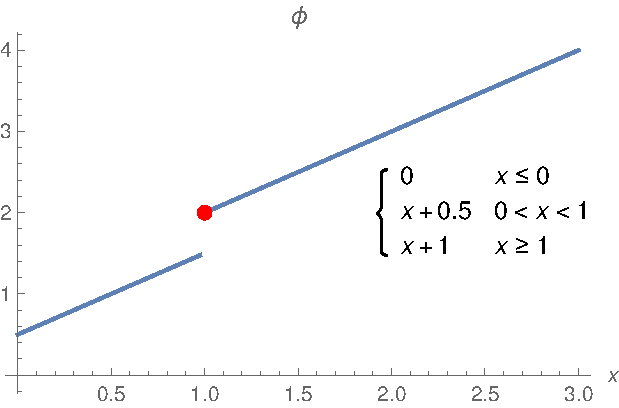
\includegraphics[height=.48\linewidth]{Chapters/example_phi.pdf}
					\caption{$d(x,y):=\phi(|x-y|)$}
				\end{minipage}
				\begin{minipage}{.49\textwidth}
					\centering
					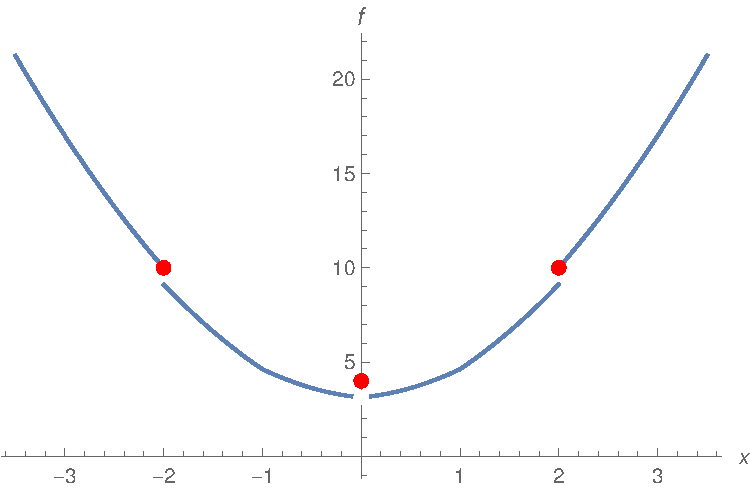
\includegraphics[height=.48\linewidth]{Chapters/example_f.pdf}
					\caption{$f(x) :=\int_{\mathbb{R}} d^2(x,y) \diff \mu(y)$}
				\end{minipage}
			\end{figure}
		\end{example}
	}
	\only<2>{
		\begin{example}[A locally compact length space but not complete]
			The unit disk with center removed.
			\\[0.3in]
			There is no barycenter for
			\begin{enumerate}
				\item uniform measure,
				\item $\frac{1}{2}\delta_x + \frac{1}{2}\delta_y$, where $x$ and $y$ center-symmetric.
			\end{enumerate}
		\end{example}
	}

	\only<3>{
		\begin{example}[A complete length space but not locally compact]
			The infinite dimensional ellipsoid with axes of length $c_n := \frac{n+1}{2n}$,
			\[
				E = \left\{ \left( x _ { 1 } , x _ { 2 } , \ldots \right) \in \ell^2 | \sum _ { n = 1}^{\infty}
				\frac { x _ { n } ^ { 2 } } { c _ { n } ^ { 2 } } = 1 \right\}.
			\]
			We consider $E$ as a smooth Hilbert Riemannian submanifold of $\ell^2$.
		\end{example}
	}
\end{frame}

\section{Wasserstein space}
\begin{frame}
	\frametitle{Wasserstein space $(\mathcal{W}(E), W)$}
	% \setbeamercovered{transparent}
	Assume $(E,d)$ is Polish:
	\textcolor{teal}{complete and separable}.

	% Consider the space

	\[
		\mathcal{W}(E): = \left\{ \mu \text{ a Borel probability measure on } E \, \left|
		\int_{E} d(x_0, y)^2 \diff \mu (y) < \infty \right. \right\}
	\]
	\pause
	% with metric $W$:
	\begin{align*}
		W ( \mu , \nu )^2
		 & = \inf \left\{ \int _ { E \times E} d ( x , y ) ^ 2 \diff \pi ( x , y )
		,\quad \pi \text{ has marginals } \mu \text{ and } \nu \right\}            \\
		 & = \inf \left\{  \mathbb{ E } d ( X , Y ) ^2
		, \quad \operatorname { law } ( X ) = \mu , \quad \operatorname { law } ( Y ) = \nu \right\}.
	\end{align*}
\end{frame}

\begin{frame}
	\frametitle{Details of Wasserstein metric $W$}
	\begin{theorem}[Existence of an optimal coupling]
		Let $(E,d)$ be a Polish space.\\
		There exists an \textcolor{cyan}{optimal coupling}
		% $(X, Y)$ with $\operatorname { law } ( X ) = \mu$ and $\operatorname { law } ( Y ) = \nu$ such that
		$\pi$ with marginals $\mu$ and $\nu$ such that
		\[
			W(\mu, \nu)^2 =
			% \mathbb{ E } d ( X , Y ) ^2.
			\int _ { E \times E} d ( x , y ) ^ 2 \diff \pi ( x , y ).
		\]
	\end{theorem}
	\pause
	To prove it, we consider \textcolor{purple}{weak convergence of measures} and show that
	\begin{enumerate}
		\item the set of all couplings is tight and
		\item the functional $\pi \mapsto \int f \diff \pi$ is lower semi-continuous.
	\end{enumerate}
\end{frame}

\begin{frame}
	\frametitle{Properties of Wasserstein space $\mathcal{W}(E)$}
	\setbeamercovered{transparent}
	Basic facts of $(\mathcal{W}(E), W)$:
	\begin{enumerate}
		\item<1> $\mathcal{W}(E)$ is a Polish space: \textcolor{teal}{complete and separable}.
		\item $(E,d)$ is a length space $\implies$ $\mathcal{W}(E)$ is a length space.
		      \item<1> $\mathcal{W}(E)$ is locally compact $\implies$ $E$ and $\mathcal{W}(E)$ are compact
	\end{enumerate}
	\setbeamercovered{invisible}
	\pause
	\begin{columns}
		\column{0.5\textwidth}
		\begin{example}[Barycenter in $\mathcal{W}(S^2)$]
			We simulate the midpoint of two uniform measures on
			the mainland shapes of China and France.
		\end{example}
		\column{0.5\textwidth}
		\begin{center}
			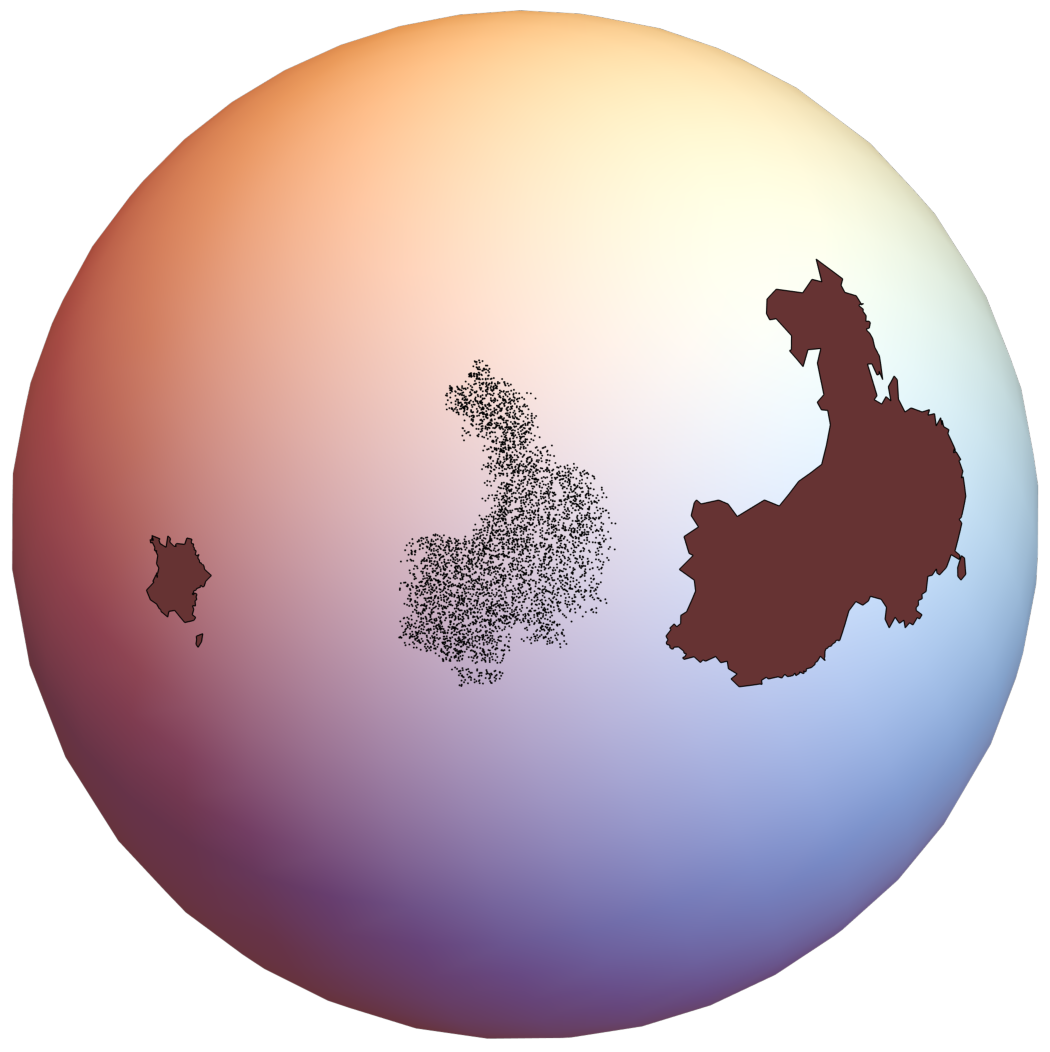
\includegraphics[width=0.5\linewidth]{Chapters/OPT_sphere.pdf}
		\end{center}
	\end{columns}
\end{frame}

\begin{frame}
	\frametitle{Barycenter's existence for
		$ \displaystyle \sum_{i=1}^n \lambda_i \delta_{\mu_i}$ on $\mathcal{W}(E)$ with $E$ proper}
	% \setbeamercovered{transparent}
	\onslide<1>{
		Let $(E,d)$ be a proper space.
		Pick $(X,X_1,\ldots,X_n)$ s.t.\@ $\operatorname{law}(X) = \mu$,
		$\operatorname{law}(X_i) = \mu_i$ and $W(\mu, \mu_i)^2 = \mathbb{E} d(X, X_i)^2$, then
	}
	\begin{equation}
		\label{equa:barycenter_selection}
		\sum_{i=1}^n \lambda_i W(\mu, \mu_i)^2 = \mathbb{E} \sum_{i=1}^n \lambda_i d(X, X_i)^2
		\geq \mathbb{E} f(X_1, \ldots, X_n),
	\end{equation}
	\onslide<1>{
		where we define}
	$ f(x_1, \ldots, x_n) := \min_{x} \sum_{i=1}^n \lambda_i d(x, x_i)^2$.
	\\[0.3cm]
	\setbeamercovered{invisible}
	\pause
	\textcolor{red}{Claim: $f$ is continous.}
	$\implies$
	\begin{enumerate}
		\item $\min \mathbb{E} f(X_1, \ldots, X_n)$ over all possible $X_i$ \pause
		\item a measurable selection $B$ from $(x_1,\ldots,x_n)$ to
		barycenters of $\sum_{i=1}^n \lambda_i \delta_{x_i}$ on $E$\\
		\onslide<5>{
			$\implies$ \emph{\textcolor{gray}{eq.\@ (\ref{equa:barycenter_selection})}} archieves an equality.
		}
	\end{enumerate}
	\setbeamercovered{invisible}
	\onslide<6>{
		Finally, barycenter \textcolor{blue}{$\bar{\mu} := B_{\#} \gamma$}, where $\gamma$
		is the law of an optimal $(X_1, \ldots, X_n)$.
	}
\end{frame}
\end{document}
